\chapter{脉搏波多维度时域特征集的构建与处理}
\section{引言}
本文第三章中已经介绍了多种描述PPG的时域特征,本章则在此基础上确定了多种基于时长、角度、斜率与面积等维度的PPG时域特征并将其作为输入用于基于机器学习的PE的识别分析之中。
与此同时,本章也将PPG信号的原始采样值也作为特殊的描述特征用于PE的识别分析。本章详细介绍了这两类特征的构建方式与处理细节。此外,本章也按机器学习的一般方法对这两类特征进行了额外的预处理工作。

\section{脉搏波多维度时域特征集的构建}
为建立识别PE的机器学习模型,本章在第三章介绍的基于PPG波形的新型时域特征的设计基础上,确定了多种新型参数的具体标准与计算方法。这些基于时长、角度、斜率与面积等维度的新型特征构成了\textbf{PPG多维度时域特征集}。
此外,本研究也将脉搏波的原始采样值视为一种特殊的PPG描述特征,将一个PPG完整波形的全部采样值视为\textbf{PPG采样值时域特征集}。
由于设计概念不同,本研究并未对以上两个PPG特征集合进行合并或交叉处理,这两个特征集合各自被\textbf{独立地}用作后续PE识别分析阶段的输入数据。

\subsection{多维度时域特征集}

在第三章已经介绍过,只要在PPG波形上的确定任意点$Q$,都可以得到与之唯一关联的一系列基于线段、曲线长度、斜率、弧度及面积等多维度时域特征,这一过程如\autoref{fig:point}所示。
从采样的角度而言,当选取了足够多的这样的基准参考点,就可以用与这些基准点关联的多维度时域特征描述PPG波形。此时,这些多维度时域特征也必然是以向量的形式存在的,也即第三章中定义的脉搏波波形特征描述向量。

因此,选取确定这些基准点的过程,是通过多维度时域特征对PPG进行描述的关键。
本研究共使用了以下三种策略确定这些基准点。\autoref{fig:all_views}也给出了三种策略的概念图。

一、左视策略

\begin{figure}[h]
  \centering
  \subfigure[\label{fig:lv}左视类指标示意]{
  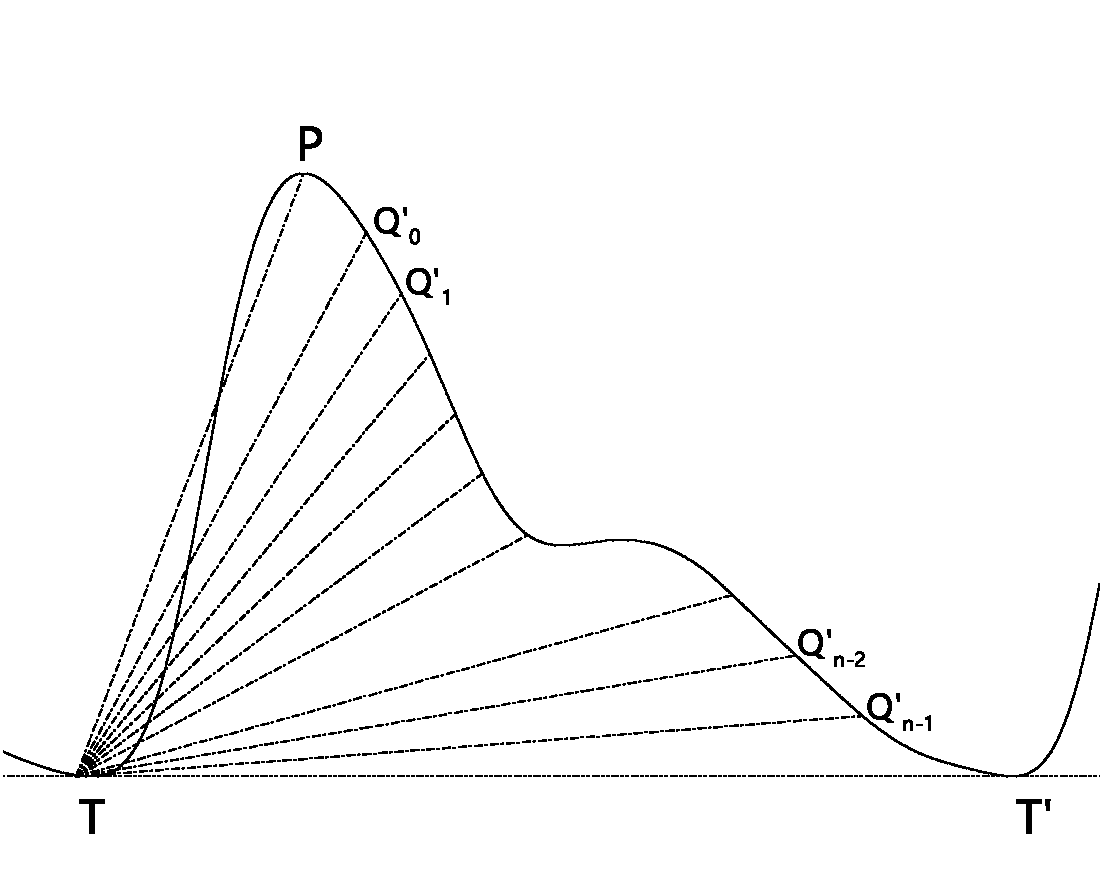
\includegraphics[width=6.5cm]{features/lv}
  }
  \quad
  \subfigure[\label{fig:cv}中视类指标示意]{
  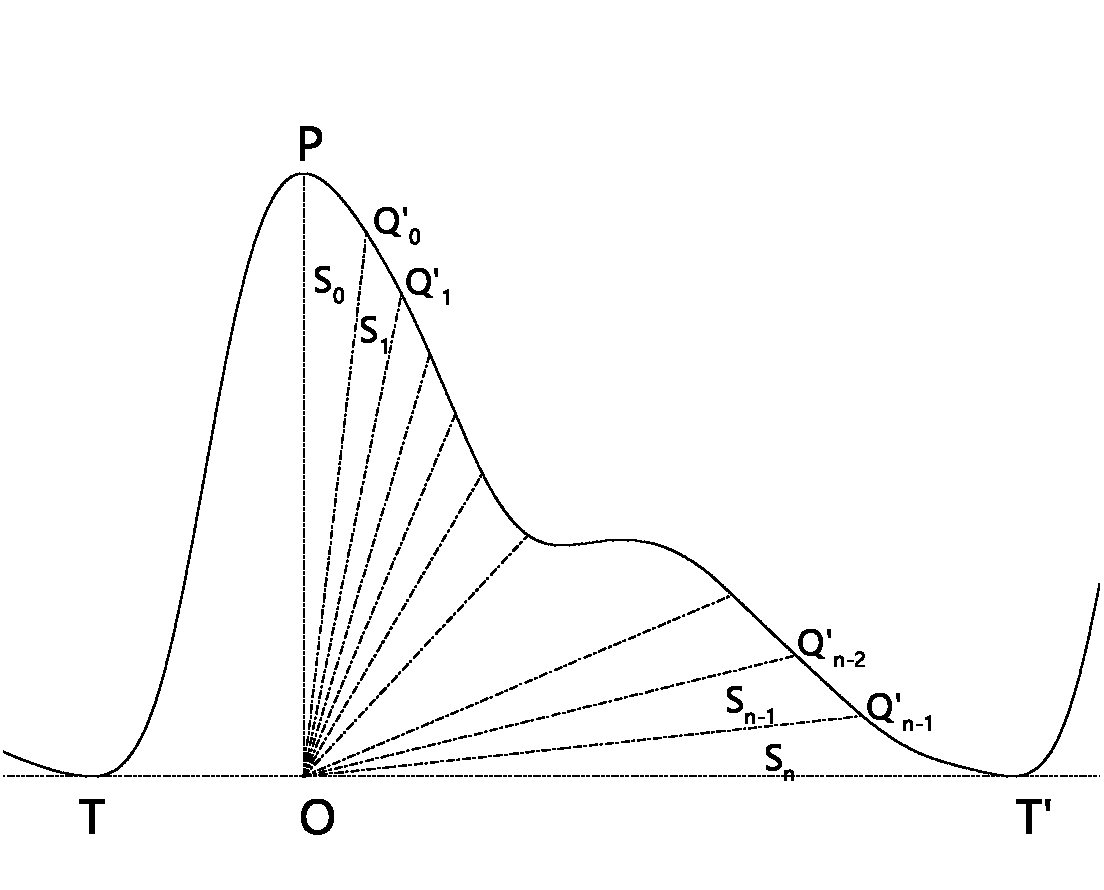
\includegraphics[width=6.5cm]{features/cv}
  }
  \quad
  \subfigure[\label{fig:sv}分层类指标示意]{
  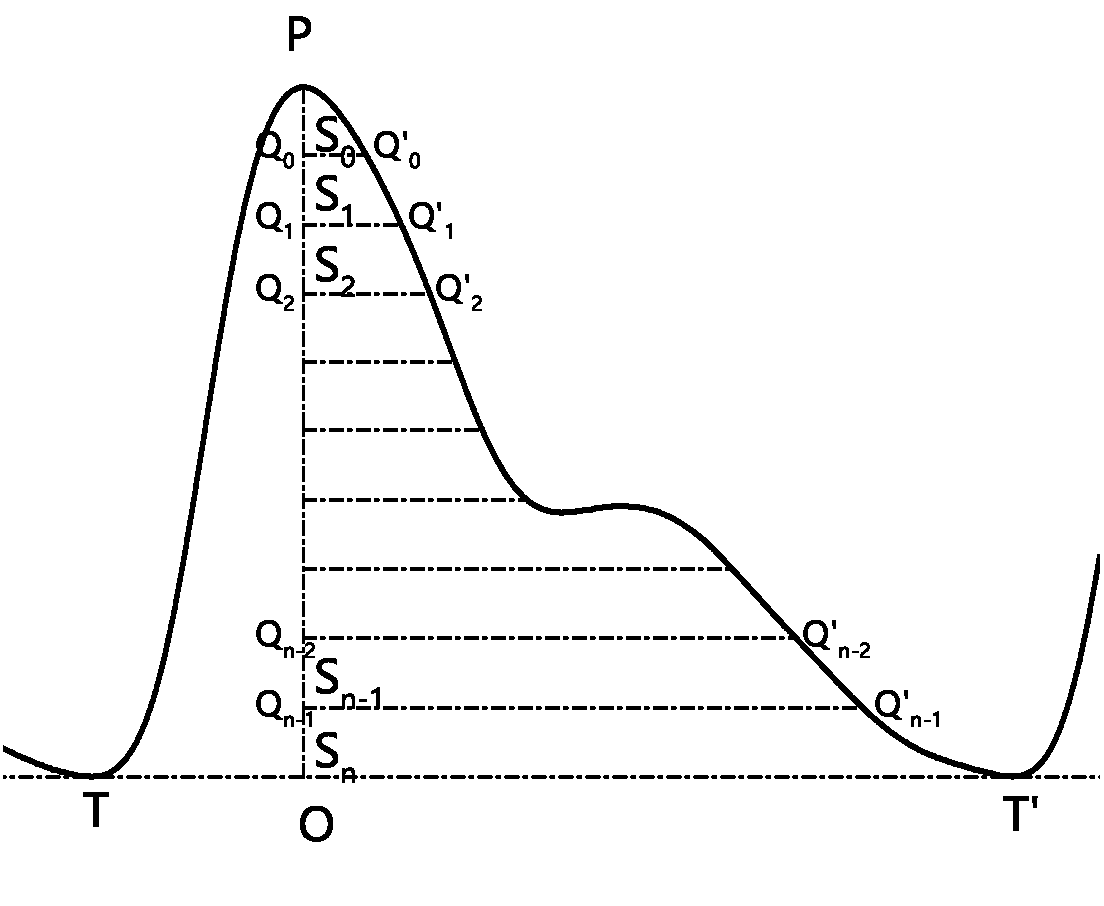
\includegraphics[width=6.5cm]{features/sv}
  }
  \caption{\label{fig:all_views}确定基准点的三种策略示意}
\end{figure}

若以PPG上升支起点为原点$T$,同时将PPG波峰设为$P$,将线段$TP$与水平基线$TT'$所构成的夹角$\angle PTT'$等分成若干份。这些等分线与PPG的交点${Q'}_i$被确定为参考基准点,这一过程如图\autoref{fig:lv}所示。由于原点被设定为PPG波形最左边的起点,本研究将这种确定基准点的方式
定义为左视策略(Left View Strategy,LVS)。

二、中视策略

若以PPG波峰$P$在水平线$TT'$上的映射点$O$为中心,将线段$OP$与水平基线构成的两个夹角$\angle POT$与$\angle POT'$等分成若干份。将这些等分线与PPG的上升支、下降支的交点计为参考基准点${Q'}_i$,这一过程如图\autoref{fig:cv}所示。由于原点被设定为PPG波峰的在水平基线上的映射点,本研究将这种确定基准点的方式
定义为中视策略(Center View Strategy,CVS)。

三、分层策略

若将PPG波峰$P$在水平线$TT'$上的映射点计为$O$,作线段$OP$的水平垂线将$OP$等分为若干份。将这些等分线与PPG的上升支、下降支的交点计为参考基准点${Q'}_i$,这一过程如图\autoref{fig:sv}所示。原点被设定为PPG波峰的在水平基线上的映射点,但为了与中视策略区分,本研究将这种确定基准点的方式
定义为分层策略(Scaled View Strategy,SVS)。


基准点的维数在本研究中也被统一设置为10,该值是在完整描述PPG的前提下避免出现信息冗余的折中选项。
经由这些策略得到的基准点最终确定得到的多维度时域特征如\autoref{tab:allfeatures}所示。
而在上述多维度时域特征计算前,PPG波形全部进行了标准化设置,波形幅值被调整缩放至[0,1000]区间内,其中PPG波形的上升支与下降支分别进行了线性变换处理。
\autoref{tab:allfeatures}也额外列举了标准化过程中涉及的斜率与截距参数。

\begin{center}
  \zihao{5}
  \begin{longtable}{m{1.5cm}<{\centering}m{3.5cm}<{\centering}m{2cm}<{\centering}m{8cm}<{\centering}}
    \caption{本研究使用的PPG多维度时域特征指标}\\
    \label{tab:allfeatures}\\
        \topline
        \colorhead \textbf{类别}&\textbf{特征名称}&\textbf{缩写符号}&\textbf{物理意义}\\
        \midline
        \endfirsthead
        \caption[]{(续)}\\
        \midline
        \colorhead \textbf{类别}&\textbf{特征名称}&\textbf{缩写符号}&\textbf{物理意义}\\
        \midline
        \endhead 
        \midline
        \endfoot
        \bottomline
        \endlastfoot
        \colorrowa &     左视斜率    &   LVS    &   各等分线所对应的直线斜率   \\
        \colorrowa &     左视上升支交点坐标 & LVLR & 等分线与PPG波形上升支交点横坐标 \\
        \colorrowa &     左视下降支交点坐标 & LVLF & 等分线与PPG波形下降支交点横坐标 \\
        \colorrowa &     左视上升支交点距离 & LVRR & 等分线与PPG波形上升支交点与波形起点距离 \\
        \colorrowa &     左视下降支交点距离 & LVRF & 等分线与PPG波形下降支交点与波形起点距离 \\
        \colorrowa &     左视交点坐标差 & LVD & 左视上升支交点坐标与左视下降支交点坐标之差 \\
        \colorrowa &     左视上升支弧长 & LVALR & PPG波形上升支被等分线分割的各区间弧长 \\
        \colorrowa \multirow{-8}*{左视策略} & 左视下降支弧长 & LVALF & PPG波形下降支被等分线分割的各区间弧长 \\
        \colorrowc &     中视上升支交点坐标 & CVLR & 等分线与PPG波形上升支交点横坐标 \\
        \colorrowc &     中视下降支交点坐标 & CVLF & 等分线与PPG波形下降支交点横坐标 \\
        \colorrowc &     中视上升支交点距离 & CVRR & 等分线与PPG波形上升支交点与峰值水平映射点距离 \\
        \colorrowc &     中视下降支交点距离 & CVRF & 等分线与PPG波形下降支交点与峰值水平映射点距离 \\
        \colorrowc &     中视交点坐标差 & CVD & 中视上升支交点坐标与中视下降支交点坐标之差 \\
        \colorrowc \multirow{-9}*{中视策略} &     中视上升支弧长 & CVALR & PPG波形上升支被等分线分割的各区间弧长 \\
        \colorrowc &     中视下降支弧长 & CVALF & PPG波形下降支被等分线分割的各区间弧长 \\
        \colorrowc &     中视上升支面积 & CVAR & PPG波形上升支被等分线分割的各区域面积 \\
        \colorrowc \multirow{-3}*{中视策略} &     中视下降支面积 & CVAF & PPG波形下降支被等分线分割的各区域面积 \\
        \colorrowa &     分层上升支交点坐标 & SVLR & 等分线与PPG波形上升支交点横坐标 \\
        \colorrowa &     分层下降支交点坐标 & SVLF & 等分线与PPG波形下降支交点横坐标 \\
        \colorrowa &     分层上升支面积 & SVAR & PPG波形上升支被等分线分割的各区域面积 \\
        \colorrowa &     分层下降支面积 & SVAF & PPG波形下降支被等分线分割的各区域面积 \\
        \colorrowa &     分层面积 & SVAT & PPG波形整体被等分线分割的各区域面积 \\
        \colorrowa &     分层上升支交点距离 & SVRR & 等分线与PPG波形上升支交点与峰值水平映射点距离 \\
        \colorrowa &     分层下降支交点距离 & SVRF & 等分线与PPG波形下降支交点与峰值水平映射点距离 \\
        \colorrowa &     分层交点坐标差 & SVD &  分层上升支交点坐标与分层下降支交点坐标之差\\
        \colorrowa &     分层上升支弧长 & SVALR & PPG波形上升支被等分线分割的各区间弧长 \\
        \colorrowa &     分层下降支弧长 & SVALF & PPG波形下降支被等分线分割的各区间弧长 \\
        \colorrowa &     分层上升支斜率 & SVSR & 等分线与PPG波形上升支交点与PPG峰值水平映射点所形成直线的斜率\\
        \colorrowa \multirow{-12}*{分层策略} & 分层下降支斜率 & SVSF & 等分线与PPG波形下降支交点与PPG峰值水平映射点所形成直线的斜率 \\
        \colorrowc &     上升支标准化斜率 & STDKR & 标准化PPG上升支波形至[0-1000]时使用的斜率 \\
        \colorrowc &     上升支标准化截距 & STDBR & 标准化PPG上升支波形至[0-1000]时使用的截距 \\
        \colorrowc &     下降支标准化斜率& STDKF & 标准化PPG下降支波形至[0-1000]时使用的斜率 \\
        \colorrowc \multirow{-4}*{标准化指标}   &  下降支支标准化截距 & STDBF & 标准化PPG上升支波形至[0-1000]时使用的截距 \\
  \end{longtable}
\end{center}

\subsection{采样值时域特征集}

前文中介绍的所有PPG特征都是基于在原始采样值的基础上通过计算间接得到的。而由于PPG信号的原始采样值本身就是对波形的量化描述,故本研究将其视为一种特殊的直接描述PPG波形的特征。
沿用本研究在第三章中的相关定义,这些采样值也可以看成是向量维数与采样点数相同的PPG波形特征描述向量。
故本研究将一个PPG完整波形的所有采样值统称为PPG采样值时域特征集,该特征集也在后续研究中被用作训练机器学习模型的输入数据。

\begin{figure}[htbp]
  \centering
  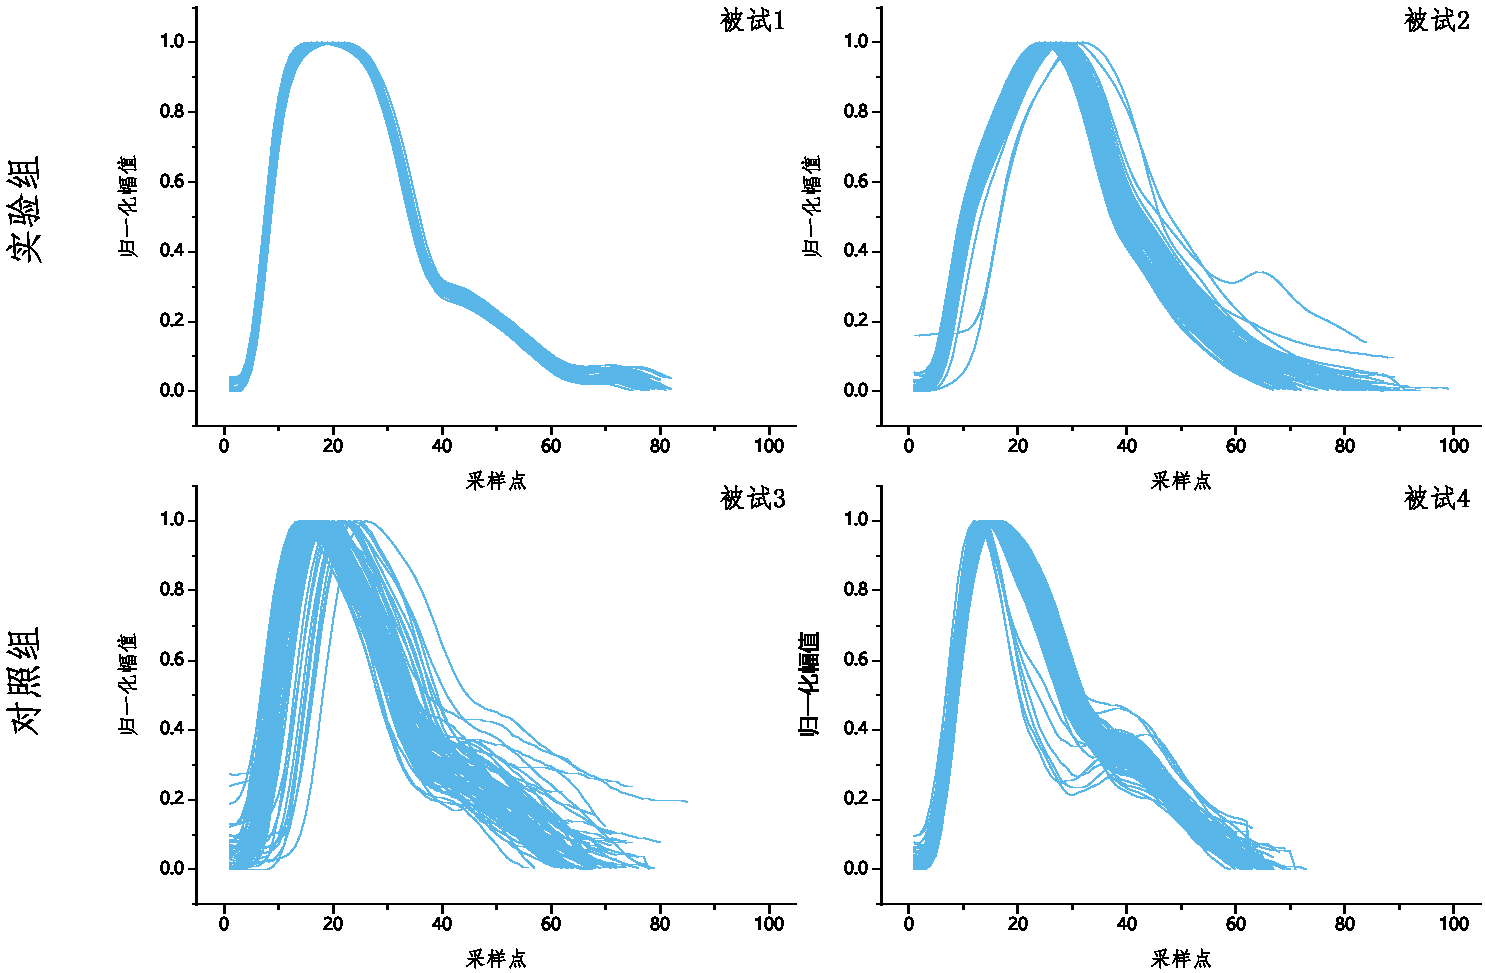
\includegraphics[width=0.75\linewidth]{features/ppgs}
  \caption{\label{fig:no_pe}被试孕妇PPG经标准化处理后的波形对照}
\end{figure}

\begin{figure}[htbp]
  \centering
  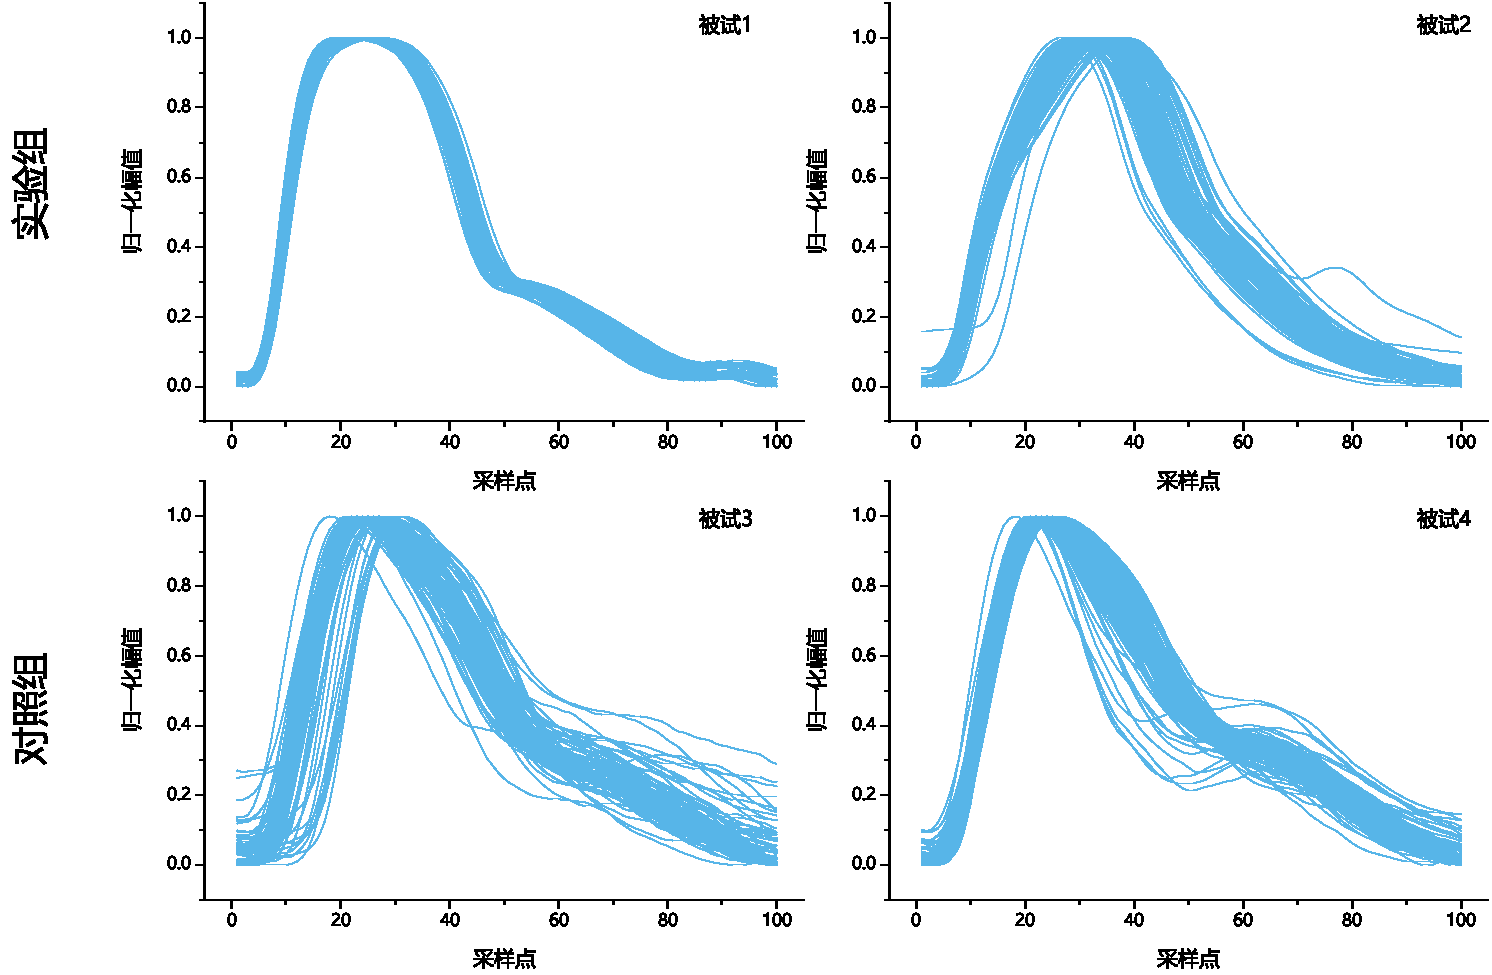
\includegraphics[width=0.75\linewidth]{features/ppgs1}
  \caption{\label{fig:no_pe2}被试孕妇PPG经标准化、重采样处理后的波形对照}
\end{figure}

对本研究的被试而言,正常组与实验组数据在PPG波形形态及整体分布上均展现了一定的差异。
\autoref{fig:no_pe}对比展示了四例被试的PPG波形差异,其中,每一幅子图在同一坐标系下绘制了同一被试的所有PPG波形,这些波形均按起点进行了对齐处理,其采样值经标准化被调整至[0,1]区间。

从\autoref{fig:no_pe}还可以看到,不同PPG波形的时长差异较为明显,在采样率固定情况下,这种差异最终会导致波形所对应的采样值时域特征集维数的差异。
为消除这种维数差异带来的影响,本研究对PPG的预处理章节介绍过的三种处理策略的适用性进行了分析,从中选取了重采样与短端补值等两种策略对PPG数据进行了处理。

一、重采样

重采样策略主要通过信号的插值与抽取将所有PPG波形的采样点数调整至相同数值$n_s$。由于采集得到的绝大多数PPG波形采样点数均不足80,本研究最终将$n_s$值确定为100。
该值保证了PPG波形的描述的分辨率与精度,同时可保证只有极少数波形需要进行采样点的压缩。
将\autoref{fig:no_pe}中的被试数据进行重采样处理,所得的最终结果如\autoref{fig:no_pe2}展示。

二、短端补齐

短端补齐策略则是以采样点数$n_e$最多的PPG波形为基准,对所有采样点不足$n_e$点的波形直接在尾端进行补零处理,使所有波形的采样点统一调整至$n_e$。
由于本研究得到的实验数据采样率为100$Hz$,本研究将$n_e$值直接设为120。与之对应的PPG波形周期也高达$1.2 s$,这一数值已经超过了本研究采集得到的任一有效的PPG波形周期。

三、长端截取

与短端补齐操作相反,长端截取策略会以采样点数$n_c$最少的PPG波形为基准,舍弃掉所有波形在$n_c$点以后的采样值。此过程不可避免地出现了数据损失,故这种策略被暂时弃用。

\section{脉搏波时域特征集的处理}
本小节明确了本论文在进行机器学习分析建模时的具体研究目标,同时也对上文中PPG时域特征集在应用于相关机器学习模型的训练之前必须进行的数据准备
工作进行了介绍。这部分内容包括数据集的划分、特征缩放及特征降维等。
\subsection{机器学习的目标}
本研究的目标是探寻PPG与PE之间的关系,即探寻使用基于PPG的数据并通过机器学习的方法识别PE的可能性。
本研究从以下两个方向展开了具体研究工作。

一、探寻被试的单个PPG波形与PE之间的关系

在此方向下,单个PPG波形被认为携带了能够表征PE患病状态的全部信息,能够作为分析识别PE的最小分析对象。同一被试的PPG数据可以对应机器学习模型训练与验证阶段的多个数据样本,这种方式相对地增加了
数据集的样本容量。

二、探寻被试的所有PPG波形与PE之间的关系

在此方向下,单个被试的所有PPG波形是作为一个整体被分析处理的,这些PPG波形的某些共性特征被认为是识别PE的关键。由于在进行数据集划分时,同一被试的PPG波形只会出现在训练集或测试集之中,
测试集中的数据样本对于训练得到的机器学习模型而言是完全陌生的。因此,这种方式更考验训练得到的模型的泛化能力。

\subsection{数据集的划分}
数据集的划分是将原始数据集划分为训练集与测试集的过程,这也是监督学习在开始模型训练前必不可少的重要步骤。其中,训练集作为训练得到特定的机器学习模型的输入,而测试集则是用来评估该模型在“新的”数据上的泛化能力。
而数据集的划分过程必须保持一定的合理性。
另一方面,针对上述两个具体目标,本研究后续章节使用了多种机器学习算法进行监督学习模型的构建。在对这些模型进行性能评估时,也必须保持数据集的划分在整个研究过程中的一致性。
因此,本研究采用了如下策略:

一、分层抽样

前人的研究已经证实,在进行数据划分时,训练集与测试集包含的样本数量最优比例在7:3\%至4:1之间\cite{Gholamy2018Why7O}。本研究按照训练集与测试集4:1的比例对原始数据抽样。
而在数据方面,本研究共采集得到79例被试孕妇的有效PPG数据波形共计7 864个,其中,44例实验组被试包含有效波形4 683个,35名对照组被试包含波形3 181个。
可以看到PPG波形数据在是否来自患有PE的实验组这一问题上存在分布不平衡现象,直接使用纯随机方法抽样有可能导致抽样偏差,最终影响准确性、稳定性与鲁棒性等模型效果\cite{Aurélien2018}。
为了避免此情况发生,本研究在构建训练集或测试集时,还额外应用了分层抽样的策略。将所有数据样本按其是否来自患有PE的实验组分成两组,对新的每组数据
分别按照4:1比例进行抽样,两组对应的抽样结果在合并之后才形成最终的训练集与测试集。

二、固化抽样结果

为保证所有模型的训练生成均基于相同的测试集,上述分层抽样结果只进行一次。随后,该划分结果不再进行任何其他调整,固化保存后供所有模型训练或测试使用。

\subsection{特征缩放}
一般而言,原始数据的输入特征在数值属性出现较大的差异会导致机器学习模型的性能下降、表现欠佳\cite{Aurélien2018}。为保证这些输入特征能满足特定的机器学习算法的输入要求,通常还要对这些特征的数值分布进行一定的调整,这也就是特征缩放操作。
常见的特征缩放处理原则是同比例缩放所有属性,使用的方法有归一化与标准化等两类。其中,归一化方法亦称为最小-最大缩放,可将所有数据的特征属性值同比例映射至[0,1]区间内。
而标准化的过程则是将所有数据的特征属性值先减去平均值后,再除以样本方差,经标准化处理得到的新数据在特征属性的数值上符合正态分布。 

\subsection{特征降维}
机器学习模型的训练过程花费的时间成本会随着输入特征维数的增加而成非线性增加,这也就是通常而言的维数诅咒或维数灾难。
为加快模型训练速度,一种可行的策略在构建模型时尽可能只使用“与预期结果最相关的”、“最重要的”输入特征,即按照特征的贡献度对
原始数据集进行降维处理。需要注意的是,数据降维在加速训练的同时,通常也会导致模型性能的下降。因此,一般认为特征降维是机器学习过程中的一个可选项而非必选项。


特征降维在训练模型前后均可进行。在训练模型前的特征降维处理
主要依赖于特征数据属性值的分布特性进行筛选;在模型训练完成后的特征降维主要依赖于特征属性对模型的贡献程度进行筛选。

本小节在训练机器学习模型前,使用U检验通过评估PPG多维度时域特征集中各特征参数与PE的相关性完成了筛选工作;在模型训练后的特征筛选处理可参见下一章节相关内容。
\autoref{tab:utest}给出了经U检验得到$p$值$>10^{-4}$的特征参数,$p$值$> 0.05$的特征未参与后续模型的训练过程,这部分特征参数在\autoref{tab:utest}进行了突出显示。

\begin{center}
  \zihao{5}
  \begin{longtable}{m{2.5cm}<{\centering}m{2cm}<{\centering}m{2.5cm}<{\centering}m{2cm}<{\centering}m{2.5cm}<{\centering}m{2cm}<{\centering}}
    \caption{脉搏波时域特征集\Rnum{1}数据特征的U检验结果}\\
    \label{tab:utest}\\
        \topline
        \colorhead \textbf{特征}&\textbf{p值}&\textbf{特征}&\textbf{p值}&\textbf{特征}&\textbf{p值}\\
        \midline
        \endfirsthead
        \caption[]{(续)}\\
        \midline
        \colorhead \textbf{特征}&\textbf{p值}&\textbf{特征}&\textbf{p值}&\textbf{特征}&\textbf{p值}\\
        \midline
        \endhead 
        \midline
        \endfoot
        \bottomline
        \endlastfoot
        \colorrowa  LVLR\_9  &  0.004 &  CVLF\_1  & \cellcolor{pink} \textbf{0.068} &  SVRR\_2  &  0.027 \\
        \colorrowc  LVLF\_1  &  \cellcolor{pink}\textbf{0.27}  &  CVLF\_2  &  0.038 &  SVRR\_3  &  0.001 \\
        \colorrowa  LVRR\_6  &  0.002 &  CVRF\_4  & \cellcolor{pink} \textbf{0.44}  &  SVRR\_4  &  0.001 \\
        \colorrowc  LVRR\_7  &  \cellcolor{pink}\textbf{0.387} &  CVD\_1   &  \cellcolor{pink}\textbf{0.159} &  SVD\_2   &  0.009 \\
        \colorrowa  LVD\_1   &  0.022 &  CVD\_2   &  0.024 &  SVD\_3   & \cellcolor{pink} \textbf{0.65}  \\
        \colorrowc  LVD\_2   &  0.006 &  CVALF\_6 &  0.02  &  SVALR\_2 & \cellcolor{pink} \textbf{0.078} \\
        \colorrowa  LVALR\_4 &  0.013 &           &        &  SVALR\_3 &  0.001 \\
        \colorrowc  LVALR\_5 &  \cellcolor{pink}\textbf{0.063} &           &        &           &               
  \end{longtable}
\end{center}

\section{小结}
本小节在已经脉搏波预处理过程的基础上完成了脉搏波时域特征集合的构建,包括基于脉搏波波形特征描述向量、原始采样值及脉搏波波形差异值等三大类。
此外,本小节也完成了机器学习的数据集划分、特征缩放及特征降维等部分的工作。